\documentclass[dvipsnames,table]{beamer}
\usepackage{polski}

\usetheme{Rochester}
\usecolortheme{orchid}

\usepackage[utf8]{inputenc}
\usepackage{listings}
\usepackage{wasysym}
\usepackage[normalem]{ulem}
\usepackage{amsmath}
\usepackage{hyperref}
\usepackage{tikzsymbols}

\setbeamertemplate{navigation symbols}{}
\setbeamertemplate{caption}[numbered]
\setbeamerfont{caption}{size=\scriptsize}
\setbeamercolor{framenote}{bg=OSEC-red!25}
\setbeamercolor{rednote}{bg=Red!25}
\setbeamercolor{palette primary}{use=structure,fg=white,bg=OSEC-red}
\setbeamercolor{palette secondary}{use=structure,fg=white,bg=OSEC-red2}

\setbeamertemplate{itemize item}{\scriptsize\raise1pt\hbox{\donotcoloroutermaths$\blacktriangleright$}}
\setbeamertemplate{itemize subitem}{\tiny\raise1pt\hbox{\donotcoloroutermaths$\bullet$}}
\setbeamertemplate{itemize subsubitem}{\tiny\raise1pt\hbox{\donotcoloroutermaths{--}}}

\setbeamertemplate{enumerate item}{\insertenumlabel.}
\setbeamertemplate{enumerate subitem}{\insertenumlabel.\insertsubenumlabel}
\setbeamertemplate{enumerate subsubitem}{\insertenumlabel.\insertsubenumlabel.\insertsubsubenumlabel}
\setbeamertemplate{enumerate mini template}{\insertenumlabel}

\setbeamercolor{itemize item}{fg=OSEC-red, bg=OSEC-red}
\setbeamercolor{itemize subitem}{fg=OSEC-red, bg=OSEC-red}
\setbeamercolor{itemize subsubitem}{fg=OSEC-red, bg=OSEC-red}

\setbeamercolor{section number projected}{fg=white,bg=OSEC-red}
\setbeamercolor{subsection number projected}{fg=white,bg=OSEC-red}
\setbeamercolor{button}{bg=OSEC-red,fg=white}
\setbeamercolor{bibliography entry author}{fg=black}
\setbeamercolor{bibliography entry title}{fg=black}
\setbeamercolor{bibliography entry location}{fg=black}
\setbeamercolor{bibliography entry note}{fg=black}

\setbeamertemplate{section in toc}[circle]
\setbeamertemplate{subsection in toc}[square]

\definecolor{OSEC-red}{RGB}{160,29,44}
\definecolor{OSEC-red2}{RGB}{177,76,12}
\hypersetup{colorlinks=true,linkcolor=white,urlcolor=OSEC-red,citecolor=black}

\setlength{\tabcolsep}{8pt}
\renewcommand{\arraystretch}{1.2}

\newcommand{\tri}{$\triangleright$ }

\newcommand\YAMLcolonstyle{\color{red}\mdseries}
\newcommand\YAMLkeystyle{\color{black}\bfseries}
\newcommand\YAMLvaluestyle{\color{black}\mdseries}

\makeatletter

\newcommand\language@yaml{yaml}

\expandafter\expandafter\expandafter\lstdefinelanguage
\expandafter{\language@yaml}
{
  keywords={true,false,null,y,n},
  keywordstyle=\color{darkgray}\bfseries,
  basicstyle=\YAMLkeystyle,                                 % assuming a key comes first
  sensitive=false,
  comment=[l]{\#},
  morecomment=[s]{/*}{*/},
  commentstyle=\color{purple}\ttfamily,
  stringstyle=\YAMLvaluestyle\ttfamily,
  moredelim=[l][\color{orange}]{\&},
  moredelim=[l][\color{magenta}]{*},
  moredelim=**[il][\YAMLcolonstyle{:}\YAMLvaluestyle]{:},   % switch to value style at :
  morestring=[b]',
  morestring=[b]",
  literate =    {---}{{\ProcessThreeDashes}}3
                {>}{{\textcolor{red}\textgreater}}1     
                {|}{{\textcolor{red}\textbar}}1 
                {\ -\ }{{\mdseries\ -\ }}3,
}

% switch to key style at EOL
\lst@AddToHook{EveryLine}{\ifx\lst@language\language@yaml\YAMLkeystyle\fi}
\makeatother

\newcommand\ProcessThreeDashes{\llap{\color{cyan}\mdseries-{-}-}}

\lstdefinestyle{yaml}
{
   language=yaml,
   basicstyle=\small\ttfamily,
   breaklines=true,
%   escapechar=\@,
}
\lstdefinestyle{bash}
{
   language=bash,
   basicstyle=\tiny\ttfamily,
   breaklines=true,
%   escapechar=\@,
}
\lstdefinestyle{cfg}
{
   basicstyle=\small\ttfamily,
   breaklines=true,
}

% bib
\begin{filecontents}{rhel8containers.bib}
@Misc{Barcamp2016,
    title = {Barcamp},
    author = {Kujawa, Radosław},
    year = {2016},
    url = {https://youtu.be/4C5cDoeSnMM?t=7703}
}
\end{filecontents}

\usepackage[style=verbose,backend=biber]{biblatex}
\addbibresource{\jobname.bib}
% end bib

\title{Konteneryzacja w Red Hat Enterprise Linux 8}
\author{Radosław Kujawa -- radoslaw.kujawa@osec.pl}
\institute{OSEC}

\begin{document}

\begin{frame}
	\titlepage
\end{frame}

\begin{frame}
\frametitle{RHEL 8 a kontenery}
	\begin{itemize}
		\item State of affairs 2019 -- konteneryzujmy wszystko niezależnie od tego, czy jest to uzasadnione, czy nie
	\end{itemize}
	\begin{center}
		
\includegraphics[scale=0.1]{img-rhlogo.png}
	\end{center}
	\begin{itemize}
		\item 8 Maja 2019 -- Red Hat Enterprise Linux 8
		\item Gdzie jest Docker?!
	\end{itemize}
\end{frame}

\begin{frame}
	\frametitle{Docker, Docker, Docker, Docker!}
	\begin{itemize}
		\item Docker jest zły i wszyscy powinniście czuć się z nim źle\footcite{Barcamp2016}
		\item {\it Security-as-an-Afterthought}
		\item Historycznie kontenery Docker działają w uprzywilejowanym namespace
		\item Architektura Dockera czyni go z definicji trudnym do zabezpieczenia
		\item Niezrozumienie wśród developerów -- Docker NIE jest mechanizmem bezpieczeństwa
		\item SELinux rozwiązuje część problemów ale za rzadko stosowany
	\end{itemize}
	\begin{center}
		
\includegraphics[scale=0.09]{img-facepalm.jpg}
	\end{center}
\end{frame}

\begin{frame}
	\frametitle{(Nie)bezpieczeństwo Dockera}
	\begin{itemize}
		\item Udokumentowana historia problemów bezpieczeństwa
		\item CVE-2019-5736 -- Docker Container Escape (btw. SELinux pomaga)
		\item Włamanie do DockerHuba, AlpineLinux z pustym hasłem roota
		\item Koszmary bezpieczeństwa -- ignorancja i złe praktyki
		\begin{itemize}
			\item Kontenery z uprawnieniami {\tt root}, {\tt CAP\_SYS\_ADMIN}
			\item Montowanie socketu Dockera wewnątrz kontenera
			\item Dostęp przez użytkowników nieuprzywilejowanych do socketu Dockera na hoście
			\item Brak polityki aktualizacji bazowych komponetnów OS wewnątrz kontenerów
		\end{itemize}

	\end{itemize}
\end{frame}

\begin{frame}
	\frametitle{Problemy innego rodzaju}
	\begin{itemize}
		\item Docker ,,standardem''? ,,Kontenery Dockerowe''
		\item rkt, LXC, systemd-nspawn?
		\item Podział Docker EE/Docker CE/Moby
		\item Moby -- upstream jednego vendora?
		\item Red Hat -- w RHEL 7 Docker ciągle patchowany (stabilność, bezpieczeństwo)
	\end{itemize}
\end{frame}

\begin{frame}
	\frametitle{Nowe narzędzia do konteneryzacji}
	\begin{itemize}
		\item Odpowiedź Red Hat, SuSE, IBM, Intel: projekt container tools \url{https://github.com/containers} 
		\item Container tools -- {\tt podman}, {\tt buildah}, {\tt skopeo} (ale nie tylko)
\end{itemize}
	\begin{center}
		
\includegraphics[scale=0.20]{img-commandos.png}
	\end{center}
\end{frame}

\begin{frame}
	\frametitle{RHEL 8?}
	\begin{itemize}
		\item Konsekwencja: RHEL 8 nie dostarcza Dockera
		\item Zastanów się 50 razy zanim zainstalujesz Docker CE -- mamy nowe narzędzia
	\end{itemize}
\end{frame}

\begin{frame}
	\frametitle{Nowy engine}
	\begin{itemize}
		\item Silnik dla kontenerów lokalnych, developmentu: podman
		\item Silnik dla dużej skali (Kubernetes, OpenShift): \href{https://cri-o.io/}{CRI-O}
	\end{itemize}
\end{frame}


\begin{frame}
	\frametitle{podman}
	\begin{itemize}
		\item Narzędzie do zarządznia lokalnymi kontenerami
		\item W pełni wspierany, to nie jest {\em tech preview}!
		\item Prostota konfiguracji, brak daemonów
		\item User namespaces -- kontenery na kontach użytkowników nieuprzywilejowanych
		\item Dobra integracja z systemd
		\item Implementacja Open Container Initiative (OCI) Runtime Specification -- obrazy zbudowane w RHEL container tools działają z Dockerem i na odwrót
		\item Ułatwienie migracji do Kubernetesa ({\tt podman generate kube, podman play kube})
		\item Dynamiczny rozwój -- RHEL 8 dostarcza {\tt podman 1.0.0}, Fedora 31 {\tt podman 1.5.1}
	\end{itemize}
\end{frame}

\begin{frame}[fragile]
	\frametitle{{\tt podman} -- integracja z {\tt systemd}}
	\begin{itemize}
		\item Kontenery {\tt podman} mogą działać jako usługi {\tt systemd}
		\item Także na koncie nieuprzywilejowanego użytkownika, w jego instancji systemd
		\item {\tt ExecStart} może uruchamiać pojedyńczy kontener lub wykonywać {\tt play kube}
		\item Mechanizm {\em socket activation} w połączeniu z kontenerami
	\end{itemize}
%\begin{lstlisting}[style=cfg]
%\lstinputlisting[style=cfg]{../podman-systemd/mycontainer.service}
% or stunnelized stdio
\end{frame}

\begin{frame}
	\frametitle{Kompatybilność wsteczna z Docker}
	\begin{itemize}
		\item Paczka {\tt podman-docker} dostarcza polecenie {\tt docker}
		\item {\tt podman} nie stara się implementować API Dockera (brak {\tt docker.sock}), jest oparty o własną bibliotekę {\tt libpod}
	\end{itemize}
\centering
	\begin{table}
\caption{Docker vs podman compatibility vs container tools native.}
\label{porownanie}
\scriptsize
\begin{tabular}{llll}
\hline
docker & rhel 8 compat & rhel 8 native   \\ \hline
	docker run & podman run & podman run \\
	docker build & podman build & buildah  \\
	docker pull & podman pull & skopeo copy \\ 
	\ldots & \ldots & \ldots \\ \hline
\end{tabular}
\normalsize
\end{table}
\end{frame}

\begin{frame}[fragile]
	\frametitle{Przykład: bc-as-a-service (build)}
\begin{itemize}
	\item Dramat plików {\tt Dockerfile}
	\item {\tt buildah} -- nowe narzędzie do budowania obrazów kontenerów
	\item Powłoka językiem skryptowania do budowy kontenerów
\end{itemize}
\lstinputlisting[style=bash]{../buildah-example/build-container.sh}
\end{frame}

\begin{frame}
	\frametitle{Przykład: bc-as-a-service (uruchomienie)}
	\begin{itemize}
		\item {\tt ./build-container.sh}
		\item {\tt mkdir -p \$HOME/tmp/logs}
		\item {\tt sudo chcon -t container\_file\_t \$HOME/tmp/logs}
		\item {\tt podman run -p 7777:7777 -v \$HOME/tmp/logs/:/logs/ localhost/bcaas}
		\item {\tt -p} dla nieuprzywilejowanych kontenerów -- libpod issue \href{https://github.com/containers/libpod/issues/2081}{2081}
	\end{itemize}
\end{frame}

\begin{frame}
\frametitle{YUM v4 (dnf) a kontenery}
\begin{itemize}
	\item microdnf -- reimplementacja {\tt dnf} o małych wymaganiach, idealna do kontenerów
%	\item Modularyzacja systemu
	\item {\em Application Streams} -- odpowiedź na potrzeby twórców aplikacji, aby dostarczać wspierane alternatywne wersje oprogramowania
	\item Ułatwia budowę kontenerów z konkretną wersją oprogramowania
	\item Pojawią się strumienie z nowszymi wersjami paczek w ramach życia RHEL 8 (np. php)
	\item Budowanie paczek zgodnie z ideologią SCL w dalszym ciągu obsługiwane
\end{itemize}
\begin{center}
\end{center}
\end{frame}

\begin{frame}
\frametitle{YUM v4 (dnf)}
\begin{itemize}
	\item Usługi, języki programowania i frameworki dostępne w alternatywnych wersjach
	\item Np. PostgreSQL 9.6 oraz 10
	\item {\tt dnf module enable postgresql:10}
	\item {\tt dnf module install postgresql:10}
\end{itemize}
\end{frame}

\begin{frame}
	\frametitle{Skopeo}
	\begin{itemize}
		\item {\tt skopeo copy source-image destination-image}
		\item Phew, that was hard
		\item Obsługiwane transporty, m.in.:
		\begin{itemize}
			\item {\tt container-storage:}
			\item {\tt dir:}
			\item {\tt docker://}, {\tt docker-archive:}, {\tt docker-daemon}
			\item {\tt oci:}
			\item {\tt ostree:}
		\end{itemize}
	\end{itemize}
\end{frame}

\begin{frame}
	\frametitle{Inne narzędzia zw. z kontenerami}
	\begin{itemize}
		\item {\tt udica} -- generator polityki SELinuxa dla kontenerów (Fedora już, RHEL 8.1+)
		\item cockpit-podman (Fedora już, RHEL 8.x)
		\item toolbox -- \url{https://github.com/containers/toolbox}
		\item \ldots 
	\end{itemize}
\end{frame}

\begin{frame}
	\frametitle{Universal Base Images}
	\begin{itemize}
		\item Oficjalne, darmowe obrazy RHEL do budowy własnych skonteneryzowanych aplikacji
		\item {\tt podman pull registry.access.redhat.com/ubi8/ubi\{,-init,-minimal\}} 
		\item {\tt podman run --rm -it ubi8/ubi /usr/bin/cat /etc/redhat-release}
	\end{itemize}
	\begin{center}
		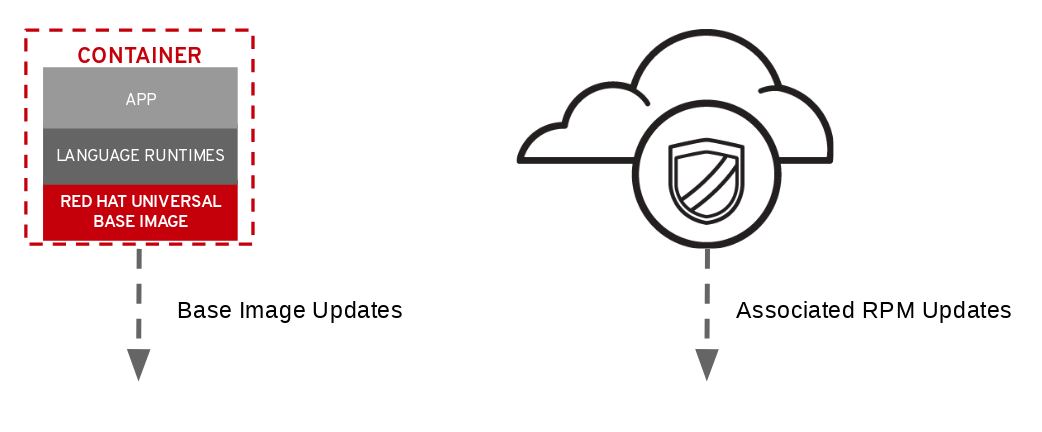
\includegraphics[scale=0.25]{img-ubiupdates.png}
	\end{center}
\end{frame}

\begin{frame}[fragile]
	\frametitle{Co z Ansible?}
	\begin{itemize}
		\item Pomysł -- Ansible jako silnik automatyzacji dla kontenerów
		\begin{itemize}
			\item Budowanie obrazów -- {\tt ansible-container}, {\tt ansible-bender}
			\item Zarządzanie kontenerami na hostach -- {\tt ansible-podman}, moduły {\tt k8s}
			\item Tworzenie skomplikowanych {\it pipelines} z kontenerami
		\end{itemize}
	\end{itemize}
\end{frame}

\begin{frame}[fragile]
	\frametitle{Budowanie obrazu kontenera za pomocą Ansible}
%	\lstinputlisting[style=yaml]{../ansible/}
\begin{itemize}
	\item {\tt ansible-bender} vs {\tt ansible-container}?
	\item {\tt ansible-bedner} nie jest jeszcze dostępny jako paczka systemowa -- jest w {\tt pip} i na GitHub
	\item {\tt ansible-bender build container-provisioning.yml}
\end{itemize}
\end{frame}

% kontenery są mechanizmem bezpieczeństwa? NIE SĄ
% są tylko mechanizmem ułatwiającym zarządzanie, oraz pozwalającym na efektywne wykorzystanie zasobów przez aplikacje

% i have no idea what I am doing


% varlink

% {\tt ansible-bender}}
%\begin{center}
%\includegraphics[scale=0.13]{img-ansibleinception.jpg}
%\end{center}
%\lstinputlisting[style=yaml,firstline=1,lastline=10]{../ansible/deploy-ansible-bender.yml}

\begin{frame}[fragile]
	\frametitle{Instalacja {\tt ansible-bender}}
	\lstinputlisting[style=yaml,firstline=11]{../ansible/deploy-ansible-bender.yml}
\end{frame}

\begin{frame}[fragile]
	\frametitle{Tworzenie obrazów kontenerów z {\tt ansible-bender}}
	\lstinputlisting[style=yaml]{../ansible/container-provisioning.yml}
\end{frame}

\begin{frame}
\frametitle{Koniec\ldots}
\begin{center}
\href{https://github.com/OSEC-pl/barcamp-osec-rhel8containers}{https://github.com/OSEC-pl/barcamp-osec-rhel8containers}

\includegraphics[scale=0.5]{img-oseclogo.png}

Dziękuje!

Czy są pytania?

\end{center}
\end{frame}
\end{document}

